\documentclass[12pt,letterpaper]{article}
\usepackage{fullpage}
\usepackage[top=2cm, bottom=4.5cm, left=2.5cm, right=2.5cm]{geometry}
\usepackage{amsmath,amsthm,amsfonts,amssymb,amscd}
\usepackage{lastpage}
\usepackage{enumerate}
\usepackage{fancyhdr}
\usepackage{mathrsfs}
\usepackage{xcolor}
\usepackage{graphicx}
\usepackage{listings}
\usepackage{hyperref}
\usepackage{amsmath}
\usepackage{mathtools}
\usepackage{tikz}
\usepackage{array}
\usetikzlibrary{matrix}

\hypersetup{%
  colorlinks=true,
  linkcolor=blue,
  linkbordercolor={0 0 1}
}
 
\renewcommand\lstlistingname{Section}
\renewcommand\lstlistlistingname{Algorithms}
\def\lstlistingautorefname{Alg.}

\lstdefinestyle{Python}{
    language        = Python,
    frame           = lines, 
    basicstyle      = \footnotesize,
    keywordstyle    = \color{blue},
    stringstyle     = \color{green},
    commentstyle    = \color{red}\ttfamily
}

\setlength{\parindent}{0.0in}
\setlength{\parskip}{0.05in}

% Edit these as appropriate
\newcommand\course{CSE 3500}
\newcommand\hwnumber{5}                  % <-- homework number
\newcommand\NetIDa{rjf23002}           % <-- NetID of person #1
\newcommand\NetIDb{}           % <-- NetID of person #2 (Comment this line out for problem sets)

\pagestyle{fancyplain}
\headheight 35pt
\lhead{\NetIDa}
\lhead{\NetIDa\\\NetIDb}                 % <-- Comment this line out for problem sets (make sure you are person #1)
\chead{\textbf{\Large Homework \hwnumber}}
\rhead{\course \\ \today}
\lfoot{}
\cfoot{}
\rfoot{\small\thepage}
\headsep 1.5em

\begin{document}

\section*{Benchmarking}

Original size of office\_hours.bmp: 2,556,834 bytes \\
Compressed using our Huffman algo: 396,887 bytes \\
Compressed using zip: 61,635 bytes \\
Compressed using rar: 43,524 bytes\\
Compressed using bzip: 26,463 bytes \\
Compressed using gzip: 60,320 bytes \\
Compression Ratio for Huffman: 6.44 \\

Original size of 1000.bmp: 3,000,054 bytes \\
Compressed using our Huffman algo: 1,030,070 bytes \\
Compressed using zip: 138,606 bytes \\
Compressed using rar: 138,793 bytes \\
Compressed using bzip: 76,900 bytes \\
Compressed using gzip: 137,048 bytes \\
Compression Ratio for Huffman: 2.91 \\

Original size of 800.bmp: 1,920,054 bytes \\
Compressed using our Huffman algo: 823,156 bytes \\
Compressed using zip: 92,719 bytes \\
Compressed using rar: 75,406 bytes \\
Compressed using bzip: 67,075 bytes \\
Compressed using gzip: 90,929 bytes \\
Compression Ratio for Huffman: 2.33 \\

Original size of 600.bmp: 1,080,054 bytes \\
Compressed using our Huffman algo: 618,236 bytes \\
Compressed using zip: 139,865 bytes \\
Compressed using rar: 163,416 bytes \\
Compressed using bzip: 92,266 bytes \\
Compressed using gzip: 136,861 bytes \\
Compression Ratio for Huffman: 1.75 \\

Original size of 400.bmp: 480,054 bytes \\
Compressed using our Huffman algo: 203,388 bytes \\
Compressed using zip: 50,862 bytes \\
Compressed using rar: 53,229 bytes \\
Compressed using bzip: 34,238 bytes \\
Compressed using gzip: 49,002 bytes \\
Compression Ratio for Huffman: 2.36 \\

Original size of 200.bmp: 120,054 bytes \\
Compressed using our Huffman algo: 67,521 bytes \\
Compressed using zip: 15,305 bytes \\
Compressed using rar: 13,776 bytes \\
Compressed using bzip: 11,961 bytes \\
Compressed using gzip: 14,550 bytes \\
Compression Ratio for Huffman: 1.79 \\

Original size of sample.txt: 90,951 bytes \\
Compressed using our Huffman algo: 34,832 bytes \\
Compressed using zip: 36,513 bytes \\
Compressed using rar: 34,957 bytes \\
Compressed using bzip: 29,563 bytes \\
Compressed using gzip: 35,836 bytes \\
Compression Ratio for Huffman: 2.61 \\

\begin{figure}[!h]
  \centering
  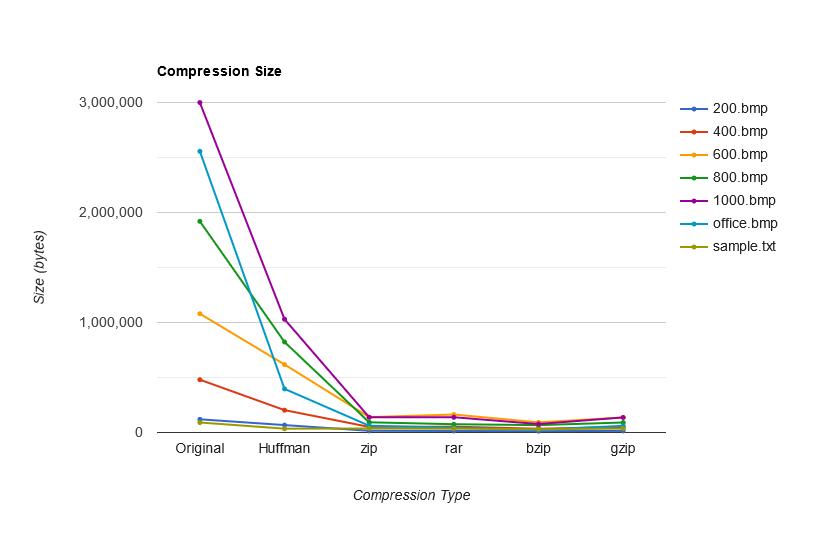
\includegraphics[width=1.0\linewidth]{line-graph.png}
  \caption{Benchmark Results}
  \end{figure}

From the data collected in the analysis,
it seems that bzip tends to give the best compression ratio due
to its tighter spread of values across different files.
The compression ratios for our Huffman algorithm tend to vary,
with outliers such as 6.44 for the office\_hours.bmp.
The typical compression ratio seems to be of at least 1.5 up till 3 times,
from the files that we sampled on. \\

However, this might be partly due to the image files that we use for testing.
In the case of office\_hours.bmp, it tends to have a lot of white pixels,
and only consisting of the colour white and black.
Potentially, the bytes may be similar such that there are lesser items in our
mapping of byte $->$ encoding, such that the encoding for each byte may 
consist of lesser number of bits.
Consequently, this affects our final compressed bitstring to have lesser total number of bits.
This may thus significantly lower the file size, resulting in a better compression ratio. \\

Compare this to the other image.bmp files, where they are mostly
made up of arbitrary colours. 
The vast difference in bytes of the file would conversely cause our mapping
to be much larger, and hence more bits are needed for each encoding.
Thus, there is a longer bit string needed for the compressed output, 
leading to a larger bytearray and thus bigger file size. \\

Thus, while our implementation of Huffman does indeed compress the file, 
more could be desired to be on par to other compression types.
For the other compression types, it can be seen that irregardless of the original file size,
the variance among the compressed outputs is usually not high. \\

Compressing sample.txt using Huffman but without BWT + MTF: 52,328 bytes \\

Yes, I do believe that BWT and MTF do help in compressing a file further.
This is because BWT first tends to group similar characters together.
MTF thus benefits from this as the output of MTF would overall have smaller values.
This is because due to the repeated property, repeated characters are generally already towards the front of the array.
Hence, the indexes of such characters would be smaller.

\end{document}
